\chapter{Background}
This chapter presents a brief overview of relevant literature on speech intelligibility, prosody, and talker familiarity.  Because the experiments described in this thesis involve speech obscured by background noise, a review of auditory masking research is also given.  The discussion of talker familiarity touches on both short-term familiarity (i.e., training and exposure studies) and long-term familiarity.  Finally, the discussion of prosody focuses on pitch, loudness, and duration as they relate to speech perception.

\section{Auditory masking}
It is well known that auditory masking is dependent on both the spectrotemporal characteristics of the masking sound as well as its relationship to the target sound.  %\citet{Miller1947} puts it succinctly: “...the masking of speech [depends] on three characteristics of the masking sound: (1) its intensity relative to the intensity of the speech, (2) its acoustic spectrum, and (3) its temporal continuity” \citep[106]{Miller1947}.  
Even the early experiments of \citet{WegelLane1924} — which involve only pure-tone targets and maskers — reveal the importance of the relationship between target and masker sounds.  Those experiments demonstrate that, regardless of the target tone frequency, masker tones \emph{close in frequency to the target tone} are the best maskers (except when the frequencies are so similar as to cause beating).  

In the nearly 90 years since, numerous aspects of the target-masker relationship have been investigated and found to impact the masking of speech.  In this section, those factors are discussed in terms of the division between energetic and informational masking, with informational masking split into two broad categories: masking due to target-masker similarity within a stimulus, and masking due to unpredictability (and, consequently, listener uncertainty) across stimuli (following \citealt{KiddEtAl2002} \latin{et seq.}).  It is acknowledged that the terms \term{energetic masking} and \term{informational masking} have historically been somewhat ill-defined \citep[cf. discussions in][]{DurlachEtAl2003a, Watson2005}, though for present purposes they will suffice as an organizing principle for review of the literature.% (since more recent terms like \term{peripheral masking} or \term{central masking} \citep{DurlachEtAl2003a} are not always obviously appropriate to describe older studies).

\subsection{Energetic and informational masking}
Early masking experiments with speech targets were often performed with noise maskers \citep[e.g.,][]{HawkinsStevens1950,Tolhurst1957b,PollackPickett1958}.  The noise used was typically a random (gaussian) signal, usually without any amplitude modulation (\term{stationary maskers}) or frequency shaping (\term{white noise maskers}).  Masking due to any such random signal is typically termed \term{energetic masking}, reflecting the idea that the masking is a consequence of elevated signal detection thresholds in the auditory filters of the cochlea (cf. the discussion in \citealt[96–97]{Moore2008}, and the notion of \term{peripheral masking} proposed by \citealt{DurlachEtAl2003a}).  However, most everyday situations involve listening to speech in the presence of competing speech streams — a situation poorly modeled by stationary white noise maskers, since real speech is both amplitude modulated and frequency shaped (indeed, the frequency shaping of speech is itself dynamic).

When speech is used as a masker, the amplitude modulations in the masker speech create temporal variations in SNR of the signal that can offer “glimpses” of the target stream \citep{FestenPlomp1990}.  The existence of such glimpses make speech a (potentially) worse masker than stationary noise, since listeners can use the glimpses to reconstruct neighboring spans of the target stream that are less clearly heard.\footnotemark{}  Glimpses can also occur with amplitude-modulated random noise maskers, and if noise maskers are both amplitude-modulated and frequency-shaped so as to be maximally comparable to speech maskers, what we find is that target perception accuracy is lower when masked by speech than by noise \citep[e.g.,][]{CarhartEtAl1969,LewisEtAl1988,SimpsonCooke2005}.  The additional masking present in speech maskers is termed \term{informational masking} (less commonly: \term{perceptual masking}), and is usually attributed to the (linguistic) information contained in the masker signal competing for language processing resources at higher levels of the auditory and language processing streams in the brain \citep{DurlachEtAl2003a,xxx}.
\footnotetext{The reconstruction of surrounding context may be based on lexical knowledge, phonotactics, transitional probabilities between words, contextual probabilities based on semantics, etc. \citep{xxx}.}

As \citet{Cooke2006} points out, glimpsing is not necessarily a strictly temporal phenomenon: there can be spectral regions of the target signal that are relatively more or less obscured by the masker signal at a given point in time.  For example, the formants of a relatively loud vowel might in fact exceed the intensity of the masker noise, especially at relatively low SNRs (see Figure~\ref{fig:PartialGlimpsing}).
%For example, a release for the alveolar stop consonant [t] typically has high levels of energy spread across the frequency range from XXX to XXX Hz \citep{xxx}.  A stationary speech-shaped noise masker might effectively mask the release burst in the frequency range from XXX to XXX, but the higher frequencies of the release burst may not be masked, offering a “partial glimpse” of the release burst, potentially recoverable by the listener as a cue to the presence of a stop consonant (see Figure~\ref{fig:PartialGlimpsing}).

\begin{figure}[htbp]
	\begin{centering}
	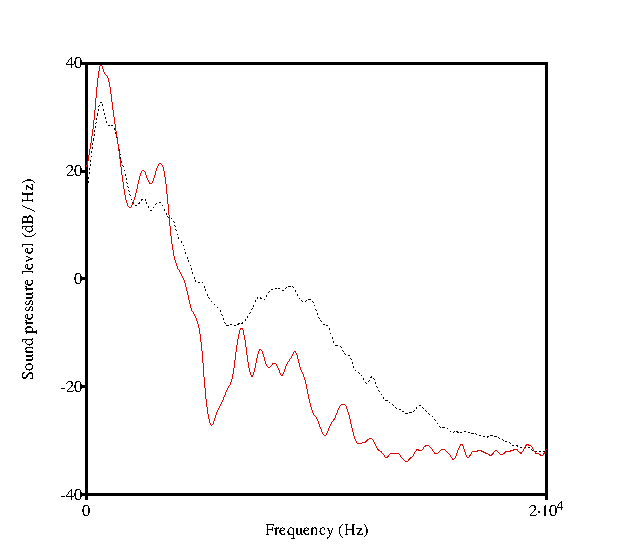
\includegraphics{partialGlimpsing.eps}
	\caption[Partial glimpsing of an {[ɑ]} vowel]{Partial glimpsing, illustrated by power spectrum of an [ɑ] vowel (solid red line) poking above the long-term average spectrum of the sentence from which the [ɑ] was extracted (dotted black line), at a signal to noise ratio of 0 dB. Both spectra have undergone cepstral smoothing with a 500 Hz bandwidth.\label{fig:PartialGlimpsing}}
	\end{centering}
\end{figure}

One can simultaneously reduce glimpses and decrease the recognizability of background speech by increasing the total number of background speech streams (i.e., by using a \term{multitalker babble masker}).  Early work by \citet{Miller1947} using babble maskers found that the degree of masking increased as the number of competing speech signals increased.  However, more recent research suggests that indefinitely increasing the number of talkers does not necessarily increase masking: total masking seems to plateau around 6–8 background talkers; further increasing the number of talkers causes the masking to recede back to the lower level seen with stationary, frequency-shaped random noise \citep{BrungartEtAl2001,SimpsonCooke2005}.  This finding can be understood as the result of an interaction between energetic and informational masking: as the number of background talkers increases, the spectrotemporal glimpses tend to decrease (increasing energetic masking), while the informational content of any individual masker voice becomes increasingly obscured by competing background talkers (decreasing informational masking).  Put another way, as the number of talkers continues to increase, spectrotemporal variation decreases and the babble masker more and more closely approximates the long-term average spectrum of speech \citep{SimpsonCooke2005}.

\subsection{Target-masker similarity\label{sec:similarity}}
Another important factor in the perception of speech in noise is the similarity of the masker and target signals.  “Similarity” may refer to fine-grained comparisons of spectral similarity (e.g., tone complexes masked by similar tone complexes, as in \citealt{LeeRichards2011}), or to more abstract properties of the signals.\footnotemark{}  As one example of a more abstract signal property, the perceived spatial origin of the competing speech streams can be construed as a form of target-masker (dis)similarity, and numerous studies have shown a release from masking due to spatial separation between the target and masker streams \citep[e.g.,][]{BrungartSimpson2002, FreymanEtAl1999, FreymanEtAl2004, KiddEtAl2005a, JohnstoneLitovsky2006}.  Likewise, \citet{Brungart2001} showed that similarity between the voices in the target and masker speech streams was also predictive of masking: perception of the target stream is most difficult when the voices in the target and masker streams belong to the same person, moderately difficult when the voices belong to same-gendered talkers, and least difficult when the target and masker voices belong to a gender-mismatched pair (a finding later replicated by \citealt{HelferFreyman2008}).
\footnotetext{Cf. the distinction in \citet{Watson2005} between target-masker \term{structural similarity} and target-masker \term{representational similarity}.}

Similarity in the language of the target and masker streams also affects masking.  For example, native English listeners perform better on English target speech when the masker speech is Spanish \citep{GarciaLecumberriCooke2006}, Dutch \citep{BrouwerEtAl2012}, or Modern Standard Chinese \citep{VanEngenBradlow2007} rather than English.  Analagous experiments by \citet{RhebergenEtAl2005} showed similar effects for Dutch listeners exposed to Dutch target speech with either Dutch or Swedish maskers.  

Informational masking also seems to be affected by the accessibility or perceptibility of the information in the masker stream(s).  For example, the release from masking seen with mismatched target and masker languages is smaller in cases where the masker language is comprehensible to the listener \citep{VanEngen2010}.  Related findings by \citet{CalandruccioEtAl2010} also support the relevance of masker accessibility or perceptibility: their study showed that for English target speech and native English-speaking listeners, native English masks better than foreign-accented English (corollary experiments confirmed that the difference was due to variation in the intelligibility of the background talker, not spectrotemporal differences between the masker streams).  Perhaps most interestingly, \citet{BrouwerEtAl2012} showed that semantically anomalous English sentences provide less masking than semantically coherent ones, but no similar effect was found for English targets masked by semantically well-formed and anomalous Dutch speech.

Taken together, these findings seem to support the view that some cases of informational masking can be explained by \term{lexical pop-out} of specific words in the masker speech \citep{HoenEtAl2007,BoulengerEtAl2010}.  According to such an explanation, comprehensible background speech can compete with target perception relatively late in the auditory processing stream (i.e., at the point at which lexemes are recognized or accessed).  In contrast (so the explanation goes), incomprehensible background speech (such as foreign-language babble) is unlikely to trigger lexical competition, except by dint of accidental similarity of foreign and native words (a very low probability occurrence).

This reasoning can be extended to the findings of \citeauthor{CalandruccioEtAl2010} showing that high-intelligibility (native) speech masks better than low-intelligibility (foreign-accented) speech, on the assumption that words are high-intelligibility precisely because they more readily trigger lexical activation (due to, e.g., greater cue redunancy).  The findings of \citeauthor{BrouwerEtAl2012} (showing weaker masking from babble comprising semantically anomalous sentences) might also be explained by appeal to lexical pop-out, though the explanation is somewhat more tenuous: a lack of semantic priming in the masker sentences would decrease the likelihood of lexical activations due to words in the masker stream, thereby reducing lexical competition from the background stream.  Regardless, many of the findings mentioned above can also be explained by appeal to stimulus uncertainty, discussed in the following section. %Moreover, the phenomenon of lexical popout presumably becomes less likely as the number of competing speech streams increases, so if differences between maskers of differing language, intelligibility, or semantic content are found with high numbers of background talkers, some other explanation must be proposed.

\subsection{Stimulus uncertainty\label{sec:uncertainty}}
Another apparent source of informational masking is the trial-to-trial regularity of the target and masker stimuli.  Experiments with pure-tone targets and pure-tone complexes as maskers have shown significant masking that is relieved when masker is held constant for the two intervals of each trial, even when the masker still varies spectrotemporally between trials \citep{NeffGreen1987, NeffCallahan1988}.  Similar results have been shown for masker spatial location \citep{FanEtAl2008} and temporal location \citep{BoninoLeibold2008}.  Such results suggest that some notion of listener uncertainty (or conversely, stimulus predictability) is important to a full account of informational masking.  Additionally, stimulus uncertainty has been shown to interact with target-masker similarity, such that masking under conditions of stimulus uncertainty is stronger when target and masker are more similar \citep{DurlachEtAl2003b}.

Experiments exploring stimulus uncertainty using speech maskers are less common, presumably due to the difficulty of controlling and quantifying the spectrotemporal similarity of speech maskers (as can be done fairly readily with tone complexes).  However, two studies using speech targets and maskers bear mentioning here.  First, it has been shown that holding the semantic content of the masker stream fixed leads to a release from masking, suggesting that masking due to listener uncertainty can arise from (semantic) variation in the masker \citep{BrungartSimpson2004}.  A second study by \citeauthor*{FreymanEtAl2007} examined the effect of listener uncertainty due to variations in SNR, talker identity in the masking stream, and constancy of masking stimulus tokens.  Surprisingly, none of these factors resulted in a significant release from masking \citep{FreymanEtAl2007}.

Despite the relative lack of research into stimulus uncertainty using speech as targets and maskers, stimulus uncertainty may play a role in explaining previous findings related to target-masker similarity.  For example, increased masking from native-language babble \citep{RhebergenEtAl2005,GarciaLecumberriCooke2006,VanEngenBradlow2007,BrouwerEtAl2012}
% PROGRESS MARKER %
%the weaker masking from semantically anomalous babble (\citealt{BrouwerEtAl2012}, mentioned in Section~\ref{sec:similarity}) 



\section{Intelligibility}

\subsection{Talker characteristics: register, clear speech, lombard effects}
Setting aside real-world situations (accommodation,etc)...  Lombard, unintentionally clear speech, intentionally clear speech, register.

\subsubsection{measurable dimensions of speech correlated with intelligibility}
\begin{itm}
	\item{loudness}
	\item{speech rate}
	\item{reduction}
	\item{vowel space}
\end{itm}

\subsection{Listener characteristics}
\subsubsection{hearing loss}
In general human auditory system looks like xxx, with little variability.  However, hearing loss, cognitive decline

\begin{itm}
	\item{target talker/listener dialect mismatch}
	\item{target talker nonnative accent}
	\item{familiarity of target voice}
	\item{native vs non-native listeners \citep{CookeEtAl2008, CookeEtAl2010, BrouwerEtAl2012}}
	\item{It has been shown that foreign babble masks less well than native babble \citep{RhebergenEtAl2005,VanEngenBradlow2007,WuEtAl2011}.  At least in some cases, native-language babble masking is due to due to distracting lexical pop-out \citep{HoenEtAl2007}.  However, it is unclear whether differences are solely attributable to lexical interference from the native background speech, or whether other aspects of the native and foreign speech might be contributing to differential masking ability (e.g., familiar vs unfamiliar phones, rhythms, or intonation contours). Rhebergen et al's study is particularly problematic, since their native-language masker (Dutch) was time-scaled using PSOLA to match the speech rate of the (unmodified) foreign-language masker (Swedish).}
	\item{priming first few words of target utterance \citep{FreymanEtAl2004}}
	\item{hearing loss}
\end{itm}

\subsection{Signal content characteristics}
\begin{itm}
	\item{redundancy}
	\item{lexical effects \citep{HoenEtAl2007, BoulengerEtAl2010, BrouwerEtAl2012}}
	\item{lexical frequency: When the masker is a speech stream, high-frequency words are more likely than low-frequency words to pop out of the background and cause distraction (i.e., slow reaction time, or mishear target word for background competitor) \citep{BoulengerEtAl2010}.}
	\item{neighborhood density}
	\item{contextual probability / predictability.  For example, \citet{LewisEtAl1988} showed that words that are predictable from context are harder to mask, in that they are recoverable (or at least guessable) at lower SNRs than the same words in low-context sentences.  At the same time, words that are predictable from context are typically articulated less distinctively, as though the talker were balancing their own articulatory effort with expectations that the listener is paying attention and can recover some words more easily than others \citep{Wright2004}.  }
	\item{Lexical activation (\textsc{aka}, word recognition) also helps when learning to recognize talkers: if the talkers are speaking an unfamiliar language, it is harder to learn to distinguish their voices \citep{PerrachioneWong2007}.}
	\item{priming target words in a simultaneous unattended contralateral speech stream \citep{RivenezEtAl2006}}
	\item{priming target talker voice and spatial location (=familiarity) \citep{KiddEtAl2005a, KitterickEtAl2010}}
\end{itm}


%A synthesis of this research leads to the conclusion that virtually every aspect of a target or masker stimulus is potentially relevant to speech perception, including many facets of speech that are often difficult to balance or control for (e.g., talker voice quality, timing of glimpses in the masker envelope, lexical frequency and semantic predictability of target words, familiarity with the talker’s voice or dialect, etc).



\section{Prosody}

\subsection{Intensity}
\begin{itm}
	\item{stress}
	\item{glimpsing}
	\item{audibility}
	\item{word-by-word SNR}
\end{itm}

\subsection{Duration}
\begin{itm}
	\item{glimpsing}
	\item{stress}
	\item{non-native duration patterns reduce intelligibility\citep{QueneVanDelft2010}}
\end{itm}

\subsection{Pitch}
\begin{itm}
	\item{creaky voicing}
	\item{spacing between harmonics, masking in that freq region}
\end{itm}

\subsection{Regional variation in prosody}

\section{Familiarity}
\subsection{Training studies}
\subsection{Long-term familiarity studies}
Newman \& Evers: college prof study\citep{NewmanEvers2007}

\subsection{Priming studies}
